\chapter{HISTORICAL BACKGROUND OF THE QUR'\=AN}\label{ch:quran_history}

The Qur'\=an (meaning \textit{the recitation}) is believed by the Muslims to have been revealed \textit{orally} by angel \arb[trans]{jibrIl} \arb{jibrIl} to Prophet Muhammad \arb{\arbmark{slm}} and passed onto other believers through oral tradition (reciting the Qur'\=an to students repeatedly so as to memorize it, instead of writing it down and let the believers read it and memorize it). Memorizing 77,429 Arabic words of the Qur'\=an through oral transmission can be a difficult task, but what aids this memorization is the rhythm feature of the Qur'\=an. According to one orientalist, \citeA{sinai2017}, "rhyme, however, or rather a periodically recurrent word-final assonance, is a feature of the Qur'\=an throughout, and it naturally partitions the \arb[trans]{sUraT} \arb{sUraT}." Indeed, because of this feature, it makes it easy to memorize the entire Qur'\=an, and the one who do so is called \arb[trans]{hafi.z} \arb{hafi.z} meaning \textit{one who remembers} or \textit{keeper}. Qur'\=an memorization contest is a common event in Muslim countries, the Philippine embassy has hosted one in 2022 in Saudi Arabia \cite{mb2022}. To support the effectiveness of the rhythmic feature on memory recall, the work of \shortciteA{lea2008} conducted three experiments using language comprehension as a framework for understanding how alliteration affects comprehension processes. Accordingly, across three experiments, alliterative cues reactivated readers' memories for previous information when it was phonologically similar to the cue. These effects were obtained when participants read aloud and when they read silently, and with poetry and prose. The results support everyday intuitions about the effects of poetry and aesthetics, and explain the nature of such effects. Further, the work of \shortciteA{lea2021rhyme} examined whether rhyme produces analogous memory-reactivation effects, and in one of their experiments participants exhibited faster recognition responses to previous poetic content as a function of rhyming cues. 

According to the Muslim tradition, the oral transmission of passing the Qur'\=an from a \arb[trans]{hafi.z} \arb{hafi.z} to new believers was gradually put into writings as requested by the believers themselves. The idea was brought up after the battle of Yamama, where many of the Muslims who died were \arb[trans]{qurrA'} \arb{qurrA'} (\textit{the one who properly recite the Qur'\=an}), and so fearing that their numbers will reduce in other battle fields, Umar ibn al-Khattab \arb{`umaru bnu 'l-xa.t.tAb} (who became the second caliph) suggested to the first caliph, Ab\=u Bakr 'Abd All\=ah ibn 'Ab\=i ibn 'Ab\=i Qu\d{h}\=afa, \arb{'abU bakriN `abdu 'l-lAhi 'ibni 'abiY qu.hAfaTa} or short for Ab\=u Bakr \arb{'abU bakr}, to collect the Qur'\=an into writing. Ab\=u Bakr then authorized Zaid ibn Thabit \arb{zaydi bni _tAbitiN} for the task. According to Zaid, he started collecting from the leafless stalks of the date-palm tree and from the pieces of leather and hides and from the stones, and from the chests of men (who had memorized the Qur'\=an, i.e. the \arb[trans]{hafi.z} \arb{hafi.z})\footnote{\textit{see} \url{https://sunnah.com/bukhari:7191}}. Long story short, the effort was finally codified by the third caliph, Uthman ibn Affan \arb{`u_tmAnu bnu `affAn} in the year 645 CE, which was then recopied and distributed to the different regional capitals of the early Islamic empire of that time. The rest of the copies outside this codification were then burned\footnote{\textit{see} \url{https://sunnah.com/bukhari:4987}} down in order to have one standard Qur'\=an. The Qur'\=an nowadays is therefore assumed to be based on Uthmanic codex because of the story mentioned. That is, if indeed Uthman has ordered to burn other copies of the Qur'\=an outside his codification, then what's left should only be based on his codex or archetype, and that should only be the inherited codex of the Muslims today.

The Qur'\=an is believed by the Muslims to have been preserved since it was first recited by angel \arb[trans]{jibrIl} \arb{jibrIl} or Gabriel to the Prophet \arb{\arbmark{slm}}. Many orientalists had been skeptic about this claim, for example, John Wansbrough theorized that the Qur'\=an was collected over a 200-year period \cite<\textit{see}>[p.~101]{wansbrough2004} after the death of the Prophet \arb{\arbmark{slm}}, instead of within a few years after the death of the Prophet \arb{\arbmark{slm}}. However, recent findings through radiocarbon dating brings forward strong evidence of potential preservation of the whole Qur'\=an, which the Muslims believed to be so. For example, the Birmingham Qur'\=an manuscript discovered in 2015 is dated to be between 568 and 645 CE with 94.5\% accuracy, making it among the oldest Qur'\=anic manuscript in the world \cite<\textit{see} >{bu2015}. Its predicted range of years intersects with the lifetime (570 to 632 CE) of the Prophet \arb{\arbmark{slm}}. What is interesting is that the Birmingham Qur'\=an is consistent with the Qur'\=an today, word-by-word and letter-by-letter\footnote{The orthography of the Arabic letters in the early days had no diacritics and were written in its basic consonantal skeleton. That is, Arabic orthography and grammar were in their nascent when the Qur'\=an was revealed, and therefore has to adjust and catch up, to capture and preserve the proper recitation of the Qur’an.}, see Figure \ref{fig:birmingham}. This is indeed another evidence that the Qur'\=an today was codified by Uthman since the discovery of the Birmingham Qur'\=an manuscripts have confirm it. In addition to this, the Sana'a Palimphest is also among the oldest Qur'\=an radiocarbon dated to be between 578 CE and 669 CE with 95\% accuracy \cite{behnam2010}, which according to \citeA{sinai2017}, "neither does the edited portion of the Sana'a palimpsest offer evidence for additional or missing verses or for a divergent verse order within the \textit{s\=urahs} \arb{sUr}." Given these discoveries on the recent Quranic manuscripts, the claim of \citeA[p.~101]{wansbrough2004} is now untenable \cite<\textit{see}>{sinai_2014}.

\begin{figure}[!b]
    \centering
    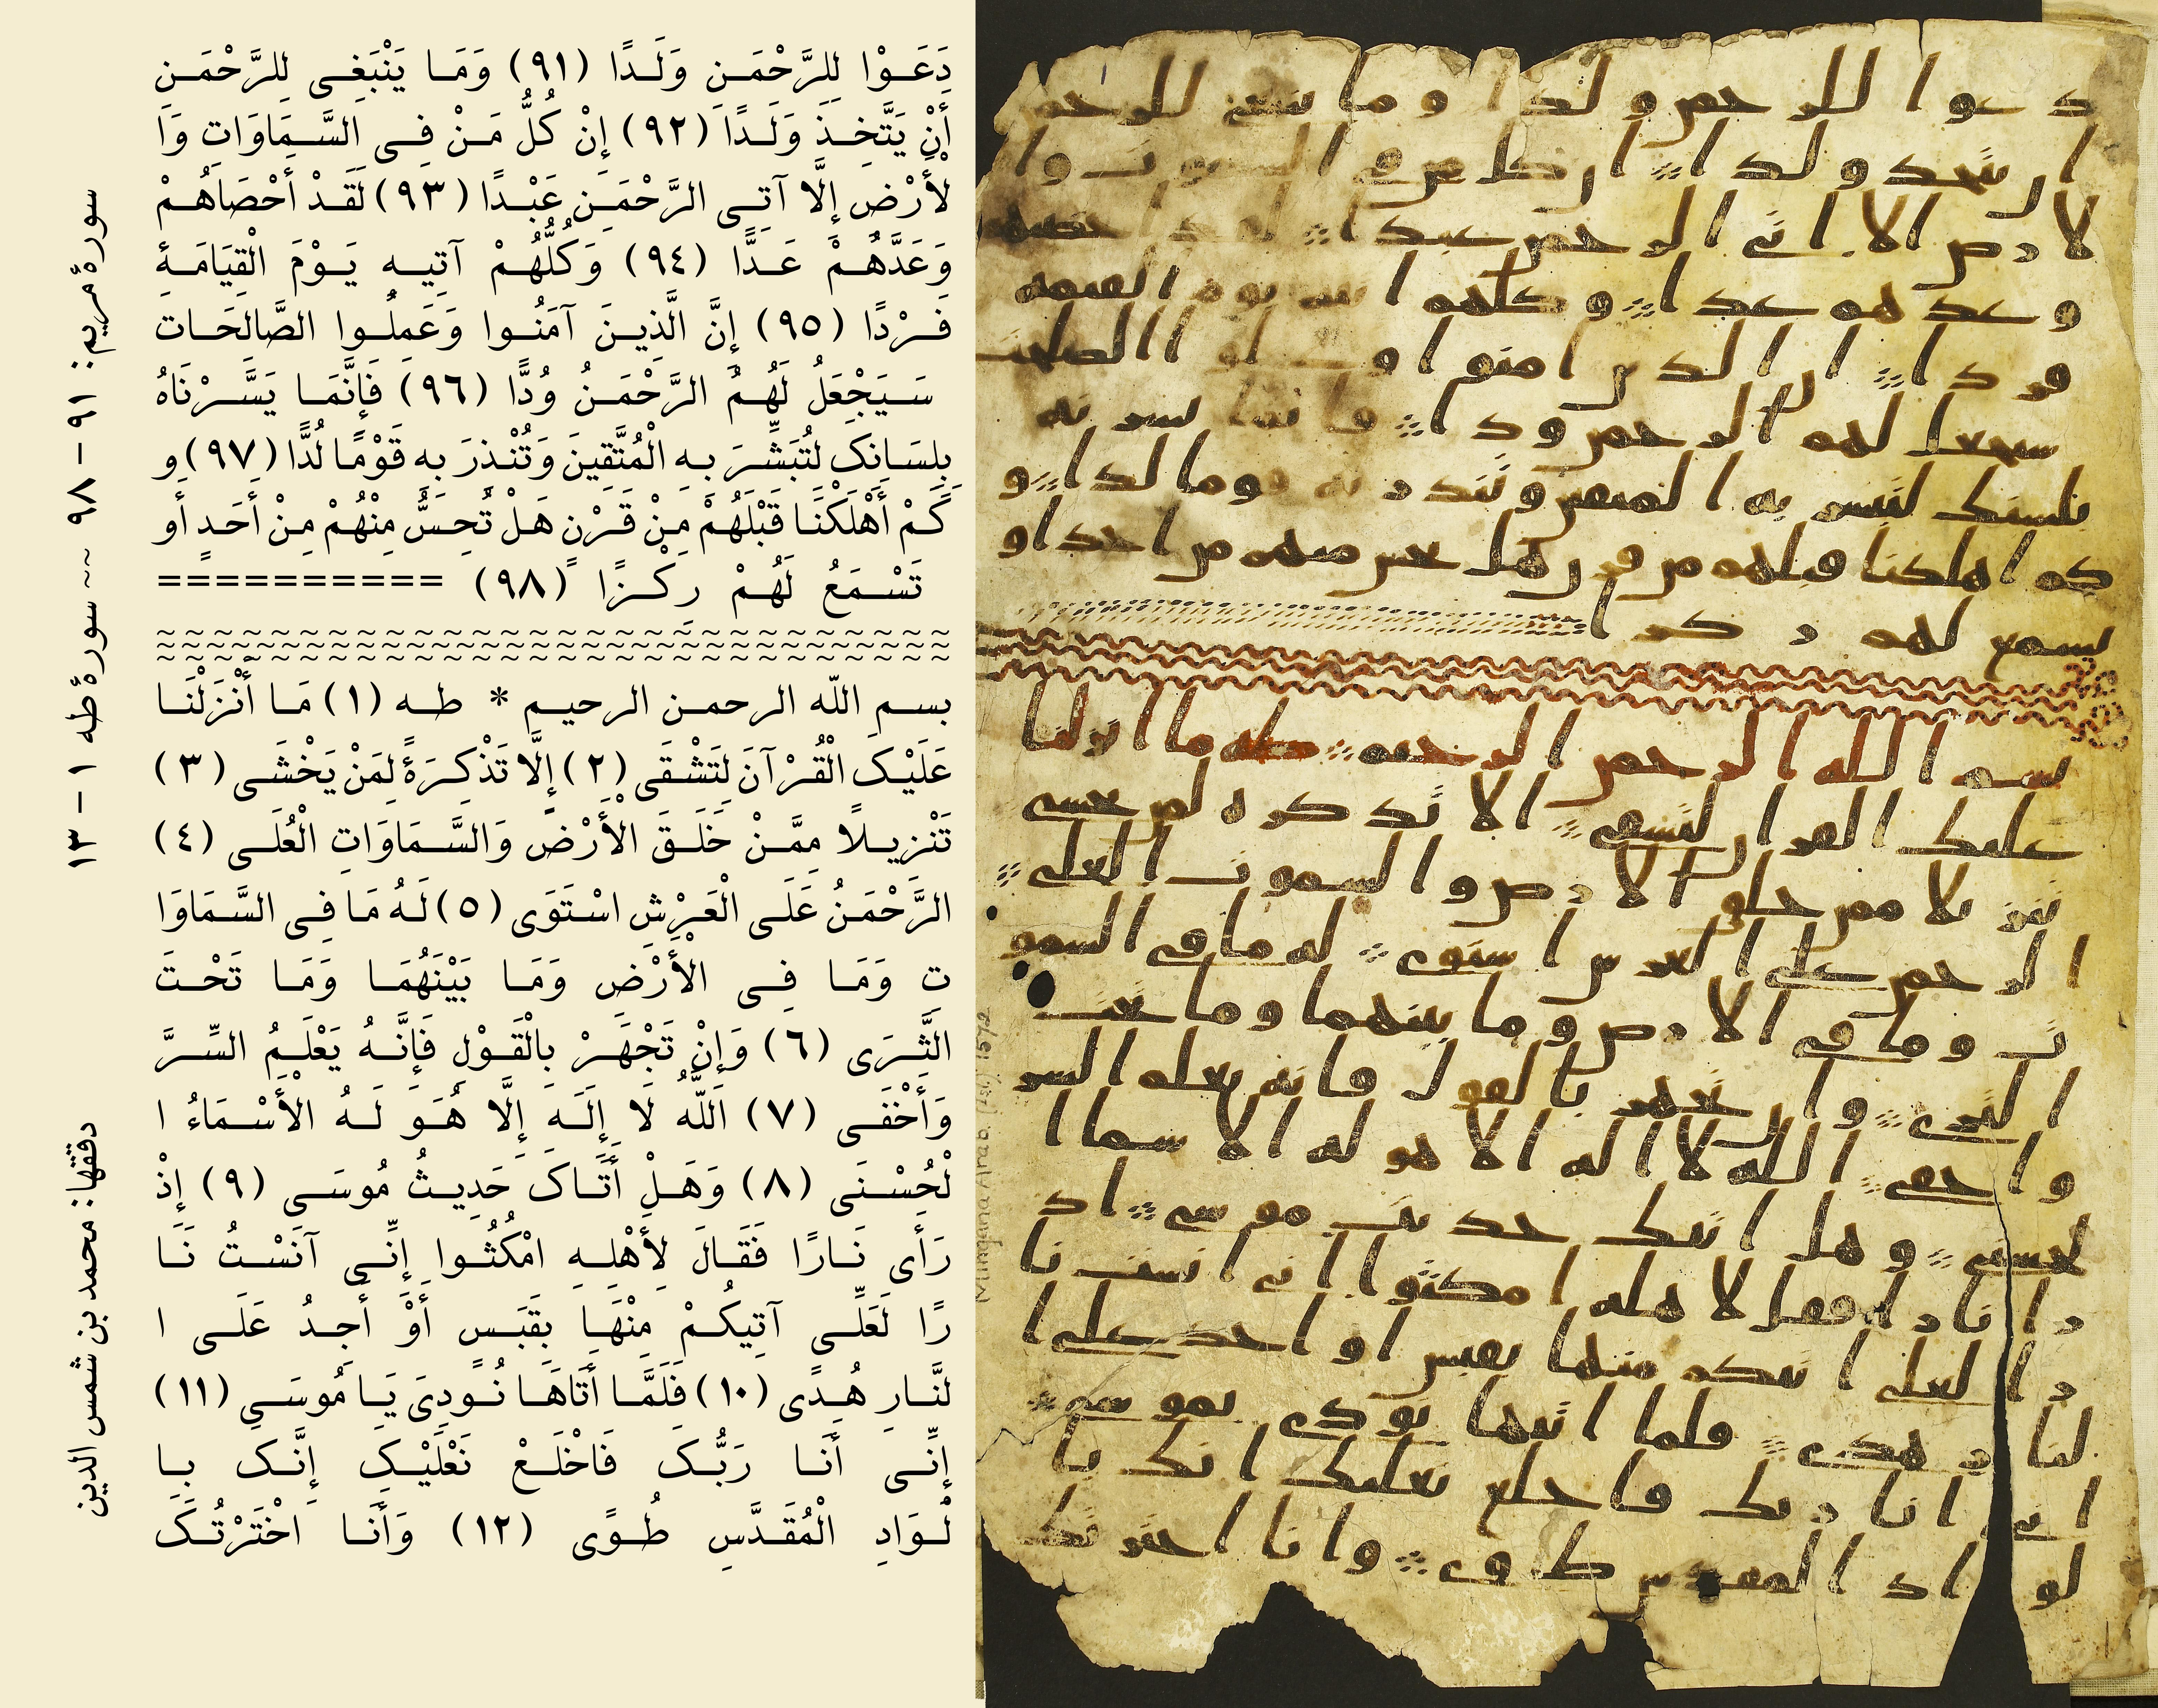
\includegraphics[width=\textwidth]{img/birmingham.jpg}
    \caption{20th Century Qur'\=an (left) in its fully featured orthographies vs Birmingham Qur'\=an dated between 568 and 645 CE (right) in its basic consonantal skeleton. Image from \protect\citeA{wikibirmingham}.}
    \label{fig:birmingham}
\end{figure}

One likely reason as to why the scribes were able to preserve the Qur'\=an in the two folios of the Birmingham Qur'\=an manuscripts follows from the fact that the Qur'\=an is firstly memorized before it was decided to be written. So that, the \mbox{Topkapi} manuscripts that contain 99\% (only 23 verses missing)---dated around 701 to 750 CE \cite{karatay1962}\footnote{\textit{see also} \url{https://corpuscoranicum.de/en/manuscripts/1977/page/1-410?sura=1&verse=1}}, that is, around 69 to 118 years after the death of the Prophet \arb{\arbmark{slm}}---of the Qur'\=an today was likely partly written from memory. This is possible since the Qur'\=an possesses a rhytmic feature (that aids with memorization) that naturally divides its verses or \arb[trans]{'ayAt} \arb{'ayAt}, and that the Qur'\=an memorization competition is still held to this day \cite<as in the example of >{mb2022}, apart from the fact that it needs to be recited (any chapter after the first chapter of the Qur'\=an according to the choice of the worshipper) every prayer from memory. Bottomline, there are many avenues for Qur'\=an recitation from memory, and these have helped in its preservation. Moreover, since there are no significant evidence of insertion or malicious intention on addition or revision in all of the extant Qur'\=anic manuscripts so far, some orientalists came up with other theories of insertions on the basis of the literary style of the Qur'\=an, see for example \citeA[p.~92]{sinai2017}, where verse 102 of \arb[trans]{sUraT 'l-.sAffAt} \arb{sUraT 'l-.sAffAt} or The Chapter of \textit{Ranged in Rows} is theorized as addition because it is longer compared to other verses in the said chapter, refer to \citeA[p.~92]{sinai2017} for his other reasonings. Some \arb[trans]{'AyAt} \arb{'AyAt}  based on this approach (tagging longer verses) of Sinai were also considered by him as plausible insertion. This paper will provide counter-argument by counter-example through early extant manuscripts. The findings as will be seen suggest that the Qur'\=an is indeed stable based on the extant manuscripts.

Furthermore, the vastness of the early Islamic empire meant that different Muslim regional capitals have covered populations with different Arabic dialects, and so to accommodate these differences, Muslims believed that there were seven variant readings of the Uthmanic codex. Variant readings are defined as different pronunciations of the same word, in this case seven Uthamnic Qur'\=an for seven different pronunciations. The \arb[trans]{.hadI_t} \arb{.hadI_t} or \textit{narration} comes from Ubayy ibn Ka'b \arb{'ubayyi bin ka`b} who reported\footnote{source: \url{https://sunnah.com/muslim:821a}} that the Prophet \arb{\arbmark{slm}} was near the tank of Banu Ghifar that \arb[trans]{jibrIl} \arb{jibrIl} or Gabriel came to him and said: "... Allah has commanded you to recite the Qur'\=an to your people in \textit{seven dialects}, and in whichever dialect they would recite, they would be right." Recent work of \citeA{sidky2020} shows that the material evidence on the regional variants is in remarkable agreement with well-attested written variants documented in the traditional Muslim literature.

Muslim and non-Muslim scholars alike have been extremely interested in understanding the unique literary characteristics of the Qur'\=an. As mentioned earlier, unlike other books like the Bible (arranged in chronological order), the Qur'\=an does not follow any obvious organization. In addition to this, a \arb[trans]{sUraT} \arb{sUraT} does not fit the exact definition of a chapter. Indeed, the name attached to a \arb[trans]{sUraT} \arb{sUraT} is often decided as the unique entity mentioned in the said \arb[trans]{sUraT} \arb{sUraT}, its main purpose is to help early Muslims distinguish which \arb[trans]{sUraT} \arb{sUraT} they are talking about, this is contrary to the chapter name where the associated name is obviously the main topic of the chapter. Further, as described by \citeA{sinai2017}, "... the compositional unity of the long surahs located at the beginning of the corpus is anything but obvious: at least at first sight, they can appear a flit back and forth between different topics in a largely haphazard manner. This impression is not limited to Western readers: even pre-modern Muslim scholars have often approached their scripture as a quarry of unconnected verses and groups of verses that bear little intrinsic relation to what precedes and follows." It wasn't until \citeA{Neuwirth_2007}, that the compositional unity of the Qur'\=an can be observed in tighter literary unities, as \citeA{Neuwirth_2007} showed that the many of these texts display a tripartite structure and are often constructive around a narrative middle part \cite{sinai2017}. Samples of the organizational style of the Qur'\=an was shown in \citeA[p.~88]{sinai2017}. Lastly, the current organization of the Qur'\=an was based on the revelations and recurring review of the Prophet Muhammad \arb{\arbmark{slm}} with the angel \arb[trans]{jibrIl} \arb{jibrIl} as believed by the Muslims. This is evident from a \arb[trans]{.hadI_t} \arb{.hadI_t} or \textit{narration} reported by Abu-Huraira in Sahih al-Bukhari saying ``Gabriel used to repeat the recitation of the Qur'an with the Prophet \arb{\arbmark{slm}} once a year, but he repeated it twice with him in the year he died. The Prophet \arb{\arbmark{slm}} used to stay in I`tikaf\footnote{I`tikaf \txarb{الاعتكاف} is a form of spiritual retreat in Islam} for ten days every year (in the month of Ramadan), but in the year of his death, he stayed in I`tikaf for twenty days.''\footnote{source: \url{https://sunnah.com/bukhari:4998}}